\chapter{Контрмера против атаки с навязыванием ключа} \label{ch:ch3}

%%%%%%%%%%%%%%%%%%%%%%%%%%%%%%%%%%%%%%%%%%%%%%%%%%%%%%%%%%%%%%%%%%%%%%%%%%%%%%%%%%%%%%%%%%%%%%%%%%%%%%%%%%%%%%%%%

\section{Атака с навязыванием ключа «поддельными» состояниями в системе квантовой коммуникации на боковых частотах} \label{sec:ch3/sec1}

 \begin{figure}[ht]
  \centering
  \includegraphics[scale=0.35]{images/scw-setup_FSA_rus1.pdf}
  \caption{Принципиальная оптическая схема предлагаемой атаки с <<поддельными состояниями>>}
  \label{fig:SCW_FSA}
\end{figure}

\pagebreak

%%%%%%%%%%%%%%%%%%%%%%%%%%%%%%%%%%%%%%%%%%%%%%%%%%%%%%%%%%%%%%%%%%%%%%%%%%%%%%%%%%%%%%%%%%%%%%%%%%%%%%%%%%%%%%%%%
\section{Границы применимости атаки с навязыванием ключа} \label{sec:ch3/sec2}

 \begin{figure}[ht]
  \centering
  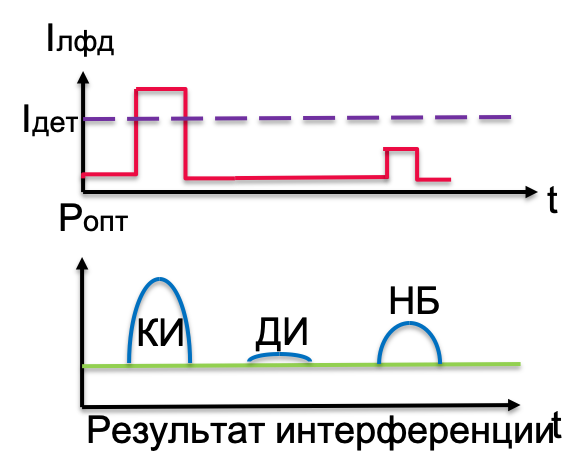
\includegraphics{Palways.png}
  \caption{Методика определения границ применимости}
  \label{fig:Palways}
\end{figure}


 \begin{figure}[ht]
  \centering
  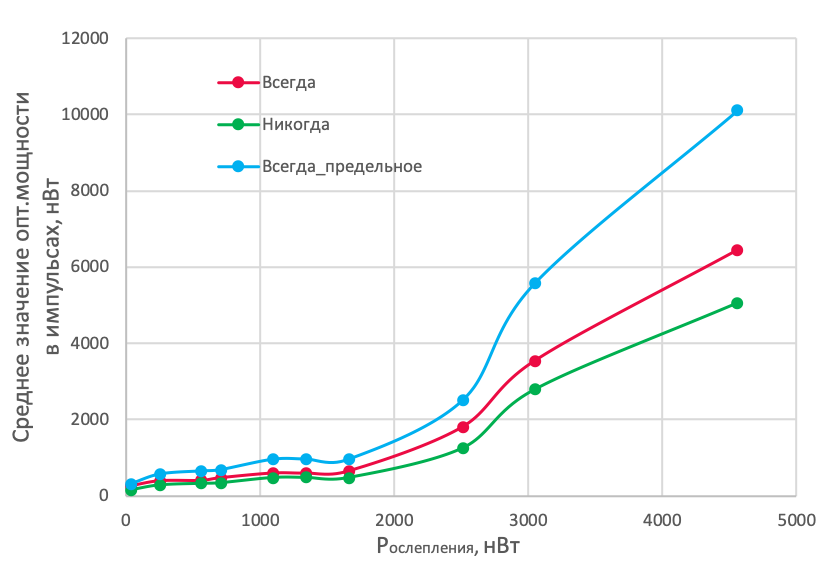
\includegraphics{Bounds.png}
  \caption{Границы применимости используемых оптических мощностей контролирующего импульса и засветки детектора}
  \label{fig:Bounds}
\end{figure}

\pagebreak

%%%%%%%%%%%%%%%%%%%%%%%%%%%%%%%%%%%%%%%%%%%%%%%%%%%%%%%%%%%%%%%%%%%%%%%%%%%%%%%%%%%%%%%%%%%%%%%%%%%%%%%%%%%%%%%%%
\section{Оценка возможностей злоумышленника при атаке с выведением детектора из режима Гейгера для систем квантовой коммуникации на боковых частотах} \label{sec:ch3/sec3}
 
 
 \begin{figure}[ht]
  \centering
  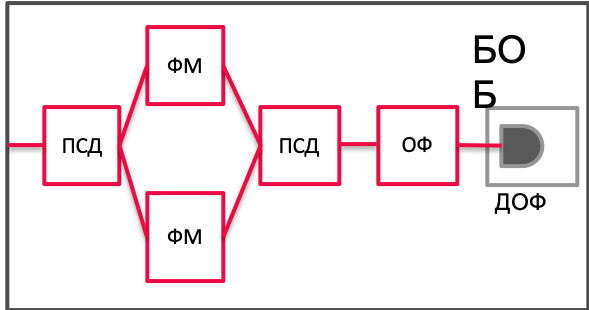
\includegraphics{Bob_scheme1.png}
  \caption{Принципиальная оптическая приемного модуля}
  \label{fig:Bob}
\end{figure}


\begin{table}
	\caption{\label{tab:blinding}Расчетные параметры для контроля детектора в системе квантовой коммуникации на боковых частотах.}
	\begin{tabular}[t]{c c c c}
	\hline\hline
	\makecell{Поддельное\\состояние\\злоумышленника\\мощность в...} & \makecell{Мощность для\\<<ослепления>> (нВт)} & $E_\text{всегда}$ (фДж) & $E_\text{никогда}$ (фДж) \\
	\hline
	\makecell{боковых после\\ фильтрации} & 35 & 25.8 & 15.4 \\
	\makecell{спектре перед\\ модуляцией} & 700 & 516 & 308 \\
	\makecell{спектре на входе\\ в приемный модуль} & 3056 & 2252 & 1345 \\
	\hline\hline
	\end{tabular}
\end{table}


\pagebreak

%%%%%%%%%%%%%%%%%%%%%%%%%%%%%%%%%%%%%%%%%%%%%%%%%%%%%%%%%%%%%%%%%%%%%%%%%%%%%%%%%%%%%%%%%%%%%%%%%%%%%%%%%%%%%%%%%

\section{Оптическая схема для противодействия атаке с <<ослеплением>> ДОФ} \label{ch:ch3/sec4}


 \begin{figure}[ht]
  \centering
  \includegraphics[scale=0.35]{images/scw-setup Countermeasure.pdf}
  \caption{Принципиальная оптическая схема предлагаемой контрмеры против атаки с <<поддельными>> состояниями}
  \label{fig:countermeasure}
\end{figure}

\pagebreak

%%%%%%%%%%%%%%%%%%%%%%%%%%%%%%%%%%%%%%%%%%%%%%%%%%%%%%%%%%%%%%%%%%%%%%%%%%%%%%%%%%%%%%%%%%%%%%%%%%%%%%%%%%%%%%%%%
\section{Экспериментальная проверка контрмеры} \label{ch:ch3/sec5}


 \begin{figure}[ht]
  \centering
  \includegraphics{images/Experimental Countermeasure.pdf}
  \caption{Принципиальная оптическая схема предлагаемой контрмеры против атаки с <<поддельными>> состояниями}
  \label{fig:Experimental_countermeasure}
\end{figure}


\pagebreak
%%%%%%%%%%%%%%%%%%%%%%%%%%%%%%%%%%%%%%%%%%%%%%%%%%%%%%%%%%%%%%%%%%%%%%%%%%%%%%%%%%%%%%%%%%%%%%%%%%%%%%%%%%%%%%%%%
\section{Динамика оптической мощности на мониторном фотодиоде}


%\[
%    \begin{cases}
%     $P_{центр}$ < 2 $P_{никогда}$ \\
%     $P_{центр}$ \geqslant  $P_{ослепления}$ 
%    \end{cases}
%\]

\[
    \begin{cases}
     $P$ < $2$ \cdot $P$ \\
     $P$ \geqslant  $P$ 
    \end{cases}
\]

 \begin{figure}[ht]
  \centering
  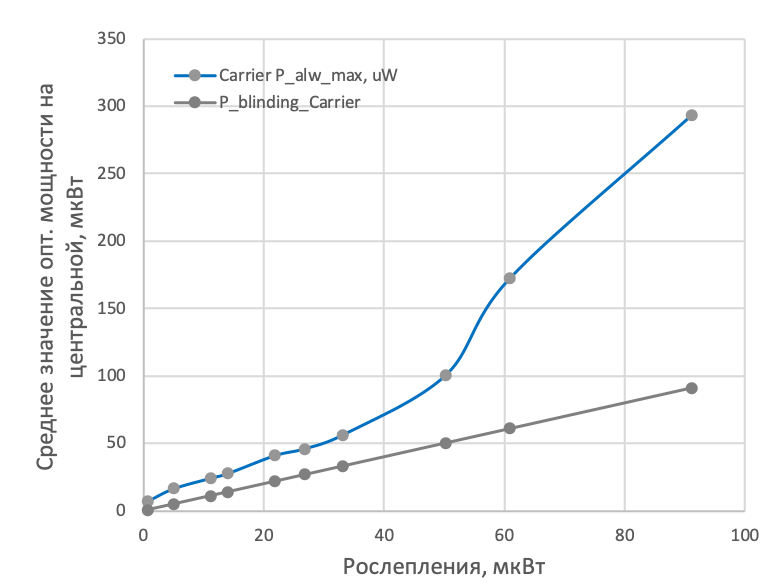
\includegraphics{images/Watchdog_photodiode.png}
  \caption{Динамика и границы оптической мощности на мониторном фотодиоде}
  \label{fig:Watchdog_photodiode}
\end{figure}


\pagebreak
%%%%%%%%%%%%%%%%%%%%%%%%%%%%%%%%%%%%%%%%%%%%%%%%%%%%%%%%%%%%%%%%%%%%%%%%%%%%%%%%%%%%%%%%%%%%%%%%%%%%%%%%%%%%%%%%%
\section{Выводы по главе} \label{ch:ch3/sect7}


Измерение величины оптического излучения на несущей частоте, отраженного от оптического фильтра, при помощи мониторного фотодиода в приемном блоке системы квантовой коммуникации на боковых частотах в диапазоне от 7 нВт до 2,93 мкВт с применением дополнительных мер в виде пассивного оптического аттенюатора номиналом 10 дБ для его защиты позволяет противостоять атаке с выведением детектора одиночных фотонов из режима Гейгера и навязыванием ключа нелегитимным пользователем. 
  